\documentstyle[color,subfigure,graphicx,epsf,here,cite,otf,comment,nccmath,mediabb,fancyhdr,12pt]{jarticle}

\graphicspath{{./pic/}}
%%%\documentstyle{jarticle}
\setlength{\textwidth}{16.2cm}%A4
\setlength{\textheight}{23cm}%A4
\setlength{\topmargin}{-1.5cm}
\setlength{\oddsidemargin}{0cm}
\setlength{\evensidemargin}{0cm}
\setlength{\parskip}{1pt}
%\pagestyle{myheadings}
\pagestyle{fancy}
\lhead[名前]{近藤徹多}
\rhead[\today]{\today}
\title{課題2 医療画像認識}
\author{近藤徹多}
\date{\today}

\begin{document}

	\maketitle
	\vspace*{20pt}

	\begin{center}
		{\LARGE \bf 基本課題}
	\end{center}
	%\setcounter{section}{0}
	\addtocounter{section}{0}
	\section{用いた手法の内容と認識率,混同行列}
	%本文
	\subsection{データ}
	訓練用画像は8980枚(正常 4486枚, 異常 4494枚), 検証画像は1448枚(正常 694枚, 異常 754枚),
	訓練用画像は2458枚(正常 1195枚, 異常 1263枚)用いた.
	図\ref{image_example}に正常画像と異常画像の例を示す.

	\begin{figure}[htbp]
		\begin{center}
			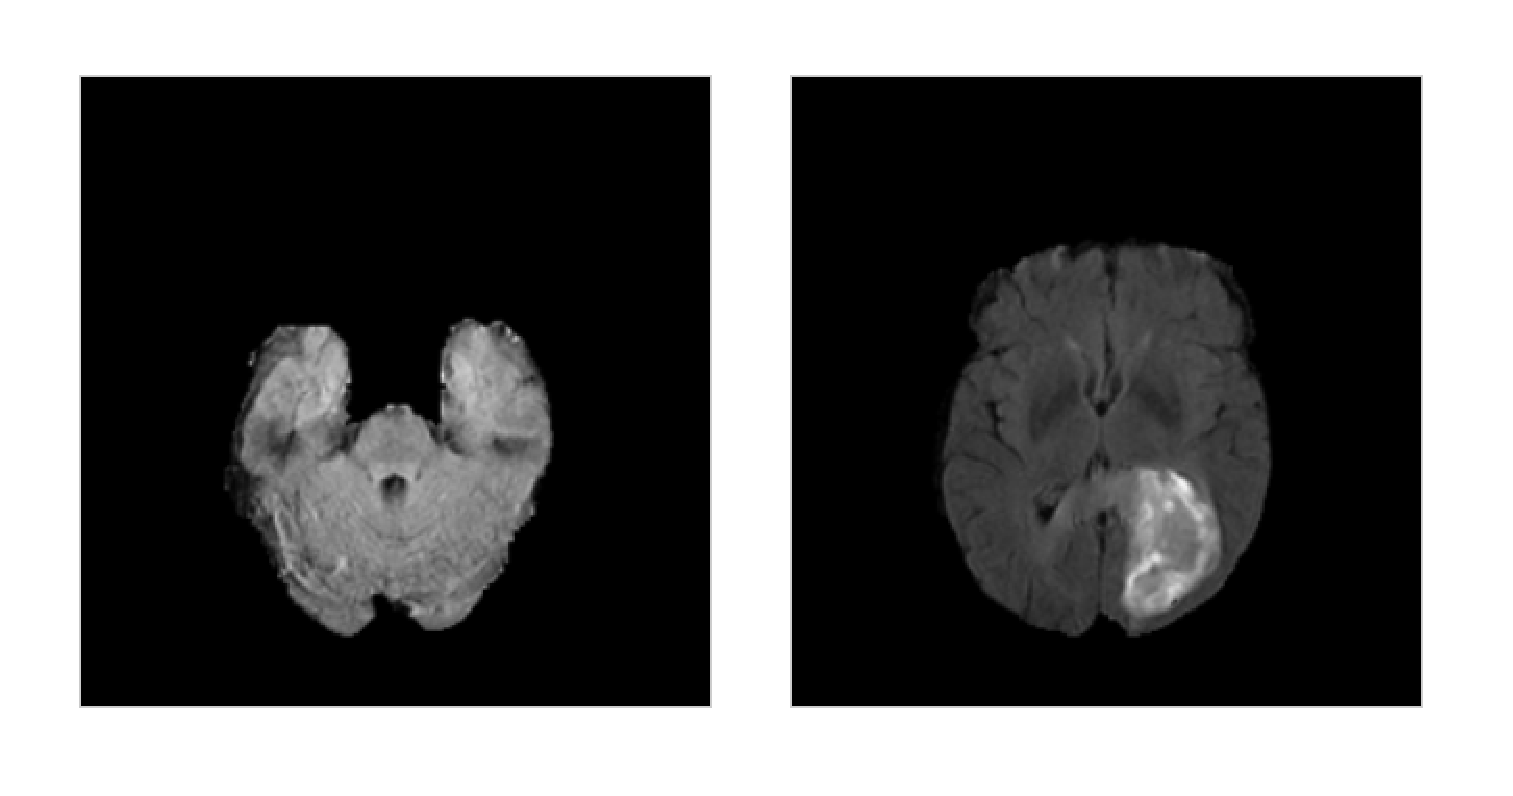
\includegraphics[width=12cm]{image_example.eps}
			\caption{正常画像(左)と異常画像(右)}
			\label{image_example}
		\end{center}
	\end{figure}


	\subsection{手法}
		医療画像の識別器としてVGG16を用いた. epoch数は50, バッチサイズは32とし,
		最適化関数はモーメンタム付きのSGDを用いて, 学習率は0.01に設定した.
		モデルのパラメータはランダムに初期化し, 全パラメータを学習した.
		また, 訓練時の画像の前処理としてランダムに水平反転を行った.


	\subsection{認識率}
		学習したVGG16を用いて, 評価用画像2458枚を識別した.
		認識率は92.0\%であった.

	\subsection{混同行列}
		混同行列を図\ref{Confusion_Matrix}に示す.
		図\ref{Confusion_Matrix}より,正常画像より異常画像のほうが誤認識しやすいことが分かる.

	\begin{figure}[htbp]
		%\begin{minipage}{\hsize}
		\begin{center}
			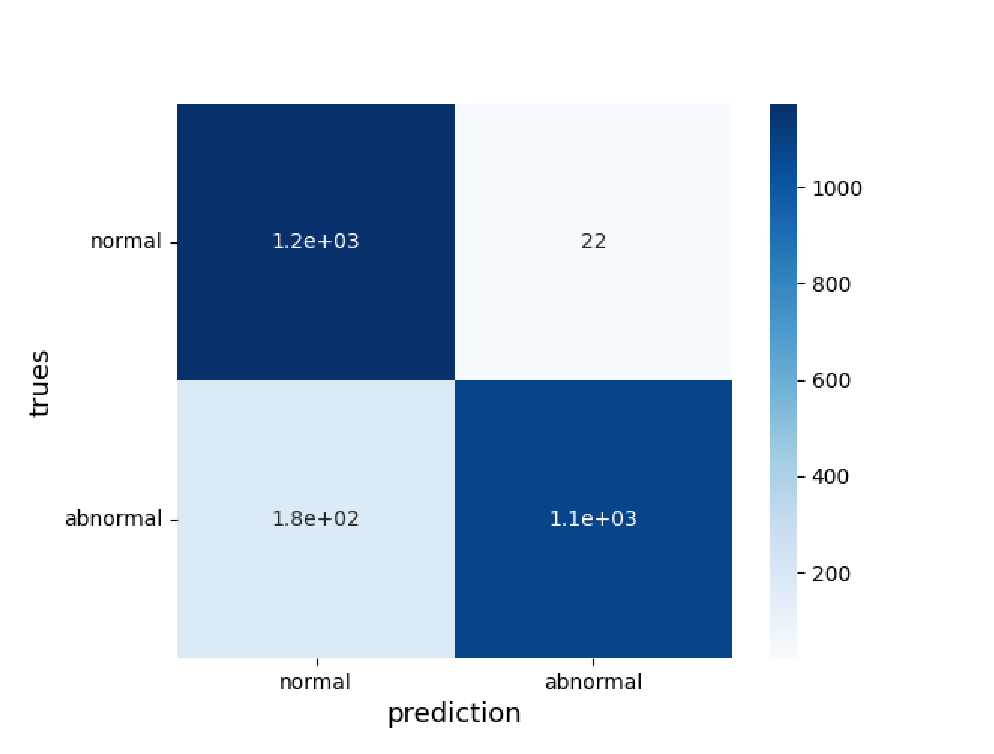
\includegraphics[width=12cm]{confusion_matrix.eps}
			\caption{混同行列}
			\label{Confusion_Matrix}
		\end{center}
		%\end{minipage}
	\end{figure}

	\newpage
	\begin{center}
		{\LARGE \bf 応用課題}
	\end{center}

	\section{正解・不正解した画像の傾向解析}
	正解した正常画像と正解した異常画像の例を図\ref{correct_example}に示す.
	正解した画像のうち, 正常画像は全体的に同じ色で構成され,
	異常画像は部分的に他と異なる色が見られ,
	図\ref{image_example}と同様の傾向が見られる.

	\begin{figure}[htbp]
		\begin{center}
			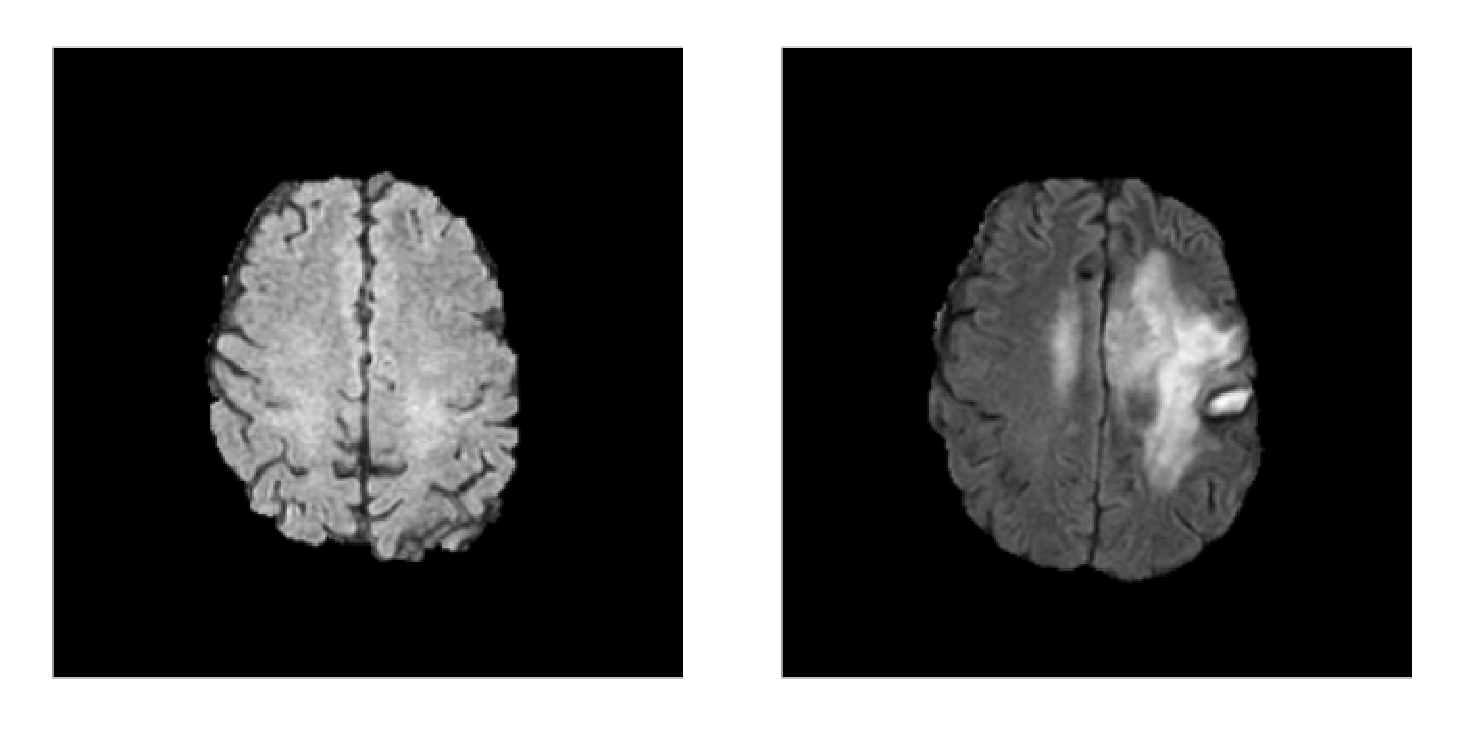
\includegraphics[width=12cm]{correct_images.eps}
			\caption{正解した正常画像(左)と正解した異常画像(右)}
			\label{correct_example}
		\end{center}
	\end{figure}

	次に, 不正解した正常画像と不正解した異常画像の例を図\ref{wrong_example}に示す.
	不正解した画像のうち, 正常画像は図\ref{image_example}の異常画像のような傾向が見られ,
	異常画像は図\ref{image_example}の正常画像のような傾向が見られる.

	\begin{figure}[htbp]
		\begin{center}
			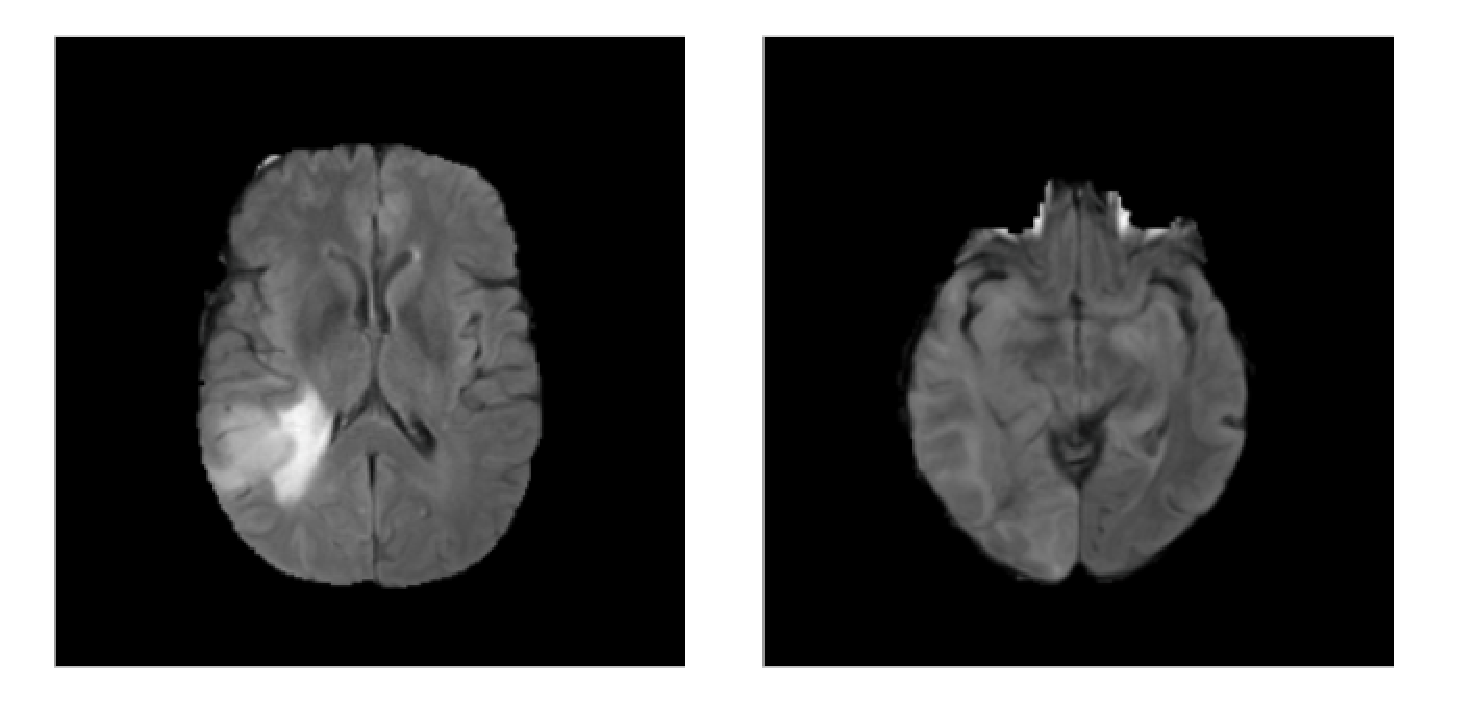
\includegraphics[width=12cm]{wrong_images.eps}
			\caption{不正解した正常画像(左)と不正解した異常画像(右)}
			\label{wrong_example}
		\end{center}
	\end{figure}


	従って, 異常画像のような傾向が見られる正常画像と正常画像のような傾向が見られる異常画像
	を正確に識別することは難しいと考えられる.

\end{document}
